\chapter{Single fiber simulations} \label{chap:three}

We explore three experiments in the context of two substrates and one fiber of reasonable length ($n=96$). The first experiment, free standing, consists of the bottom substrate and a ``free standing'' fiber. Free standing in the sense that any buckled configuration for a set of parameters is not in principle caused by the load applied to the top substrate.

The second experiment, compression, adds the top substrate with some associated applied load. We measure the adhesion of particles of the fiber to particles of the top substrate and observe equilibrium configurations. The question of adhesion for these experiments is only relevant for a fiber particle in relation to a particle on one of the substrates. Thus we have the following heuristics,
\begin{eqnarray} \label{eqn:adhesion}
	A(\textbf{a}, \textbf{b}) = \left\{ 
		\begin{array}{ll}
			1, & \|\textbf{a} - \textbf{b}\| \leq 1.1 \sigma + 10^{-6}\\
			0, & \mbox{otherwise}
		\end{array}
		\right.  \\
	A_+ = \sum_{k=1}^{n^+} \sum_{j=1}^{m} \sum_{i=1}^{n} A(\textbf{r}_i^{(j)},\textbf{r}_k^{(+)}) \label{eqn:adhesion:top} \\ 
	A_- = \sum_{k=1}^{n^-} \sum_{j=1}^{m} \sum_{i=1}^{n} A(\textbf{r}_i^{(j)},\textbf{r}_k^{(-)}). \label{eqn:adhesion:bottom}
\end{eqnarray}
The equilibrium distance between any two particles is $\sigma$, however we relax this distance by $10\%$ and a numerical translation to take into account simulation precision.

The third experiment, detachment, consists of a fiber buckled only at the root and entirely adhered to both the top and bottom substrates. Adhered in the sense that every fiber particle will satisfy (\ref{eqn:adhesion}). A load is applied to the top substrate in an attempt to break an adhesive contact with the fiber. With all three experiments we focus primarily on equilibrium configurations. The heuristic (\ref{eqn:adhesion}) is then used as a method of categorizing different equilibrium configurations for varying parameters.

\section{Free standing}

We say a fiber, or part of a fiber, is \textit{crystallized} if the van der Waals energy between a collection of fiber particles appears qualitatively to be minimized. This is precisely the notion of adhesion we use for fiber particles in relation to substrate particles. Crystallization of a fiber is however a more global effect. If a fiber is going to crystallize at one location the same mechanism will cause crystallization elsewhere until several, if not all, particles on the fiber are in a crystallized state. 

	\begin{figure}[ht!]
		\begin{center}
			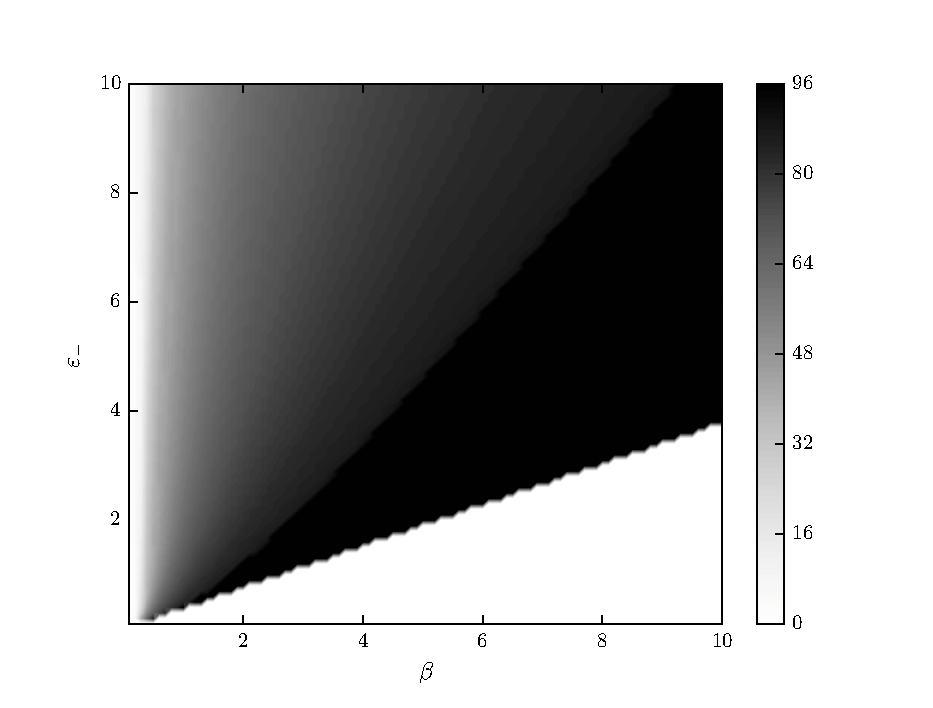
\includegraphics{./fig/ch3/fs/grid.eps}
		\end{center}		
		\caption{Plot of torsional spring strength, $\beta$, by bottom substrate vdW strength, $\eps_-$, colored by adhered (fiber) particle count to the bottom substrate. There are three distinct regions that categorize the behavior of a fiber: the black region of flattened fibers, the white region of standing or slanted fibers, and the grey sub-regions.
		\label{fig:fs}}
	\end{figure}

We say a fiber is \textit{flattened} if every particle of the fiber is adhered to the bottom substrate. If the parameters of the system are such that a fiber will be flattened in the free standing experiment then it would be difficult for the top substrate to have any influence on altering the fiber's configuration. In both the compression and detachment experiment we are more interested in parameters that do not give a flattened configuration. Therefore, it is pertinent to categorize for what parameters a fiber is flattened or not. In this regard we conjecture that the torsional spring and vdW interaction between the fiber and bottom substrate are critical and fiber to fiber vdW interaction or extensible springs are negligible.

	%% Fallen Figures
	\begin{figure*}[h!]
		\centering
		\begin{subfigure}{.5\textwidth}
			\centering
			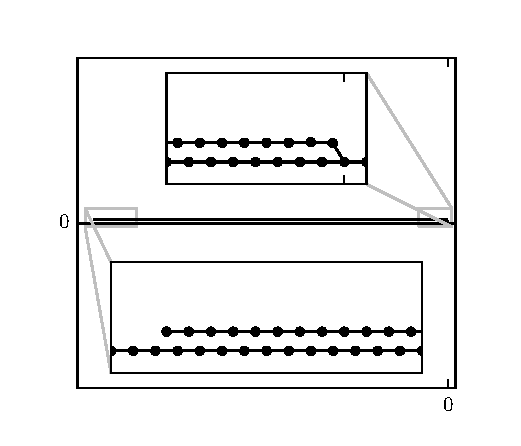
\includegraphics{./fig/ch3/fs/b5_eb3.eps}
			\caption{$\beta=5$ and $\eps_-=3$.\label{subfig:lazy}}
		\end{subfigure}%
		~
		\begin{subfigure}{.5\textwidth}
			\centering
			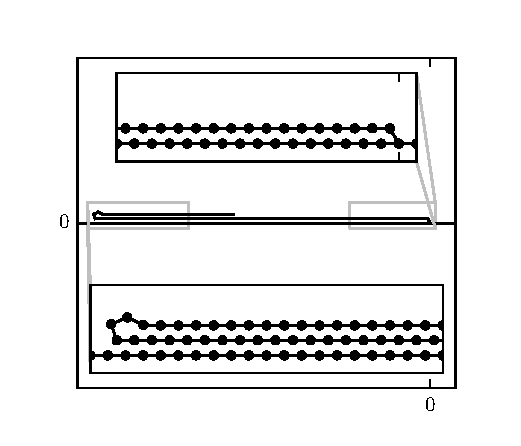
\includegraphics{./fig/ch3/fs/b2_eb6.eps}
			\caption{$\beta=2$ and $\eps_-=6$.\label{subfig:lazy_loop}}
		\end{subfigure}

		\begin{subfigure}{.5\textwidth}
			\centering
			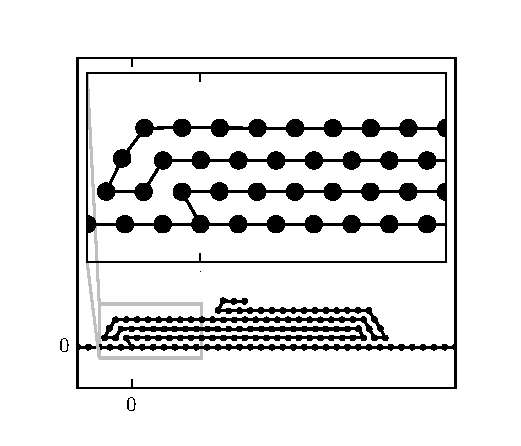
\includegraphics{./fig/ch3/fs/b0.5_eb10.eps}
			\caption{$\beta=0.5$ and $\eps_-=10$.\label{subfig:lazy_many_loops}}
		\end{subfigure}		
		\caption{The black region of Figure~\ref{fig:fs} consists strictly of (a) flattened fibers. (b) Configurations that contain a single kink are located in the grey region near the black region. (c) Configurations with additional kinks are located farther away.\label{fig:lazy}}	
	\end{figure*}

Varying $\beta$ and $\eps_-$ is shown in Figure~\ref{fig:fs} colored by fiber adhesion with the bottom substrate. The black region of the plot corresponds to flattened configurations, and only flattened configurations (see Figure~\ref{subfig:lazy}). If there is any buckling in the fiber a particle would be too far away to be considered adhered. 

	%% Erect Figures
	\begin{figure*}[t!]
		\centering
		\begin{subfigure}{.5\textwidth}
			\centering
			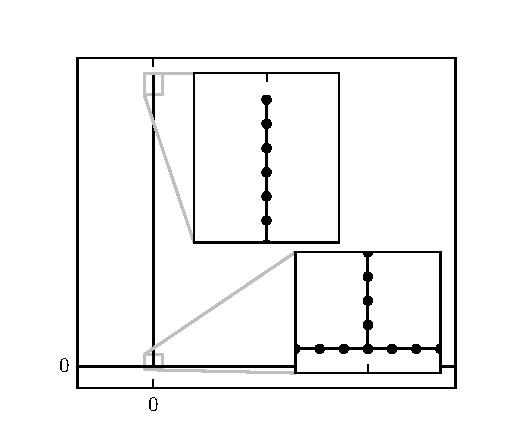
\includegraphics{./fig/ch3/fs/b10_eb1.eps}
			\caption{$\beta=10$ and $\eps_-=1$.\label{subfig:erect}}
		\end{subfigure}%
		~
		\begin{subfigure}{.5\textwidth}
			\centering
			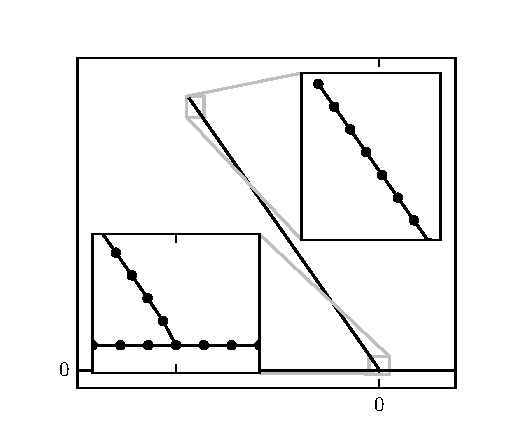
\includegraphics{./fig/ch3/fs/b10_eb3.eps}
			\caption{$\beta=10$ and $\eps_-=3$.\label{subfig:leaning}}
		\end{subfigure}
		\caption{The white region of Figure~\ref{fig:fs} consists strictly of standing fibers. A standing fiber does not need to be (a) orthogonal to the bottom substrate, but can be (b) slanted and straight or curved.\label{fig:alert}}
	\end{figure*}

	%% Crystalized Figures
	\begin{figure*}[h!]
		\centering
		\begin{subfigure}{.5\textwidth}
			\centering
			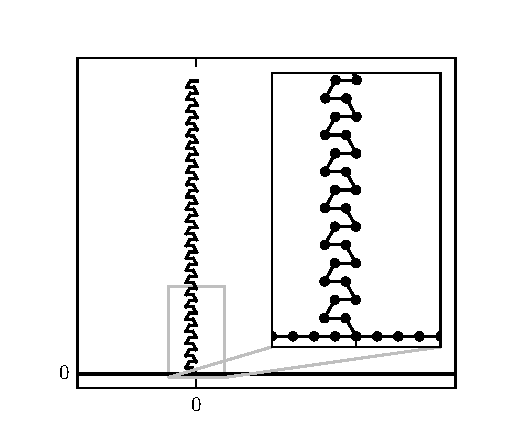
\includegraphics{./fig/ch3/fs/b0.1_eb0.5.eps}
			\caption{$\beta=0.1$ and $\eps_-=0.5$.\label{subfig:hex_chain}}
		\end{subfigure}%
		~
		\begin{subfigure}{.5\textwidth}
			\centering
			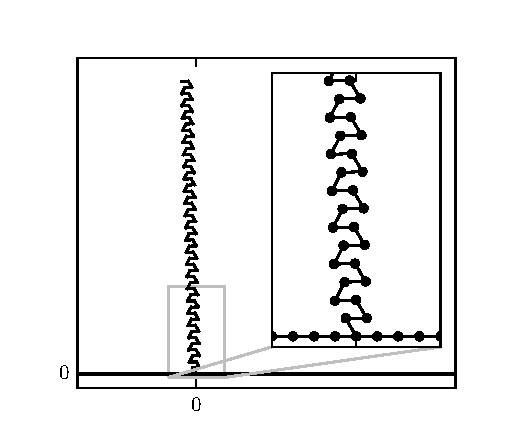
\includegraphics{./fig/ch3/fs/b0.1_eb3.eps}
			\caption{$\beta=0.1$ and $\eps_-=3$.\label{subfig:leaning_hex_chain}}
		\end{subfigure}

		\begin{subfigure}{.5\textwidth}
			\centering
			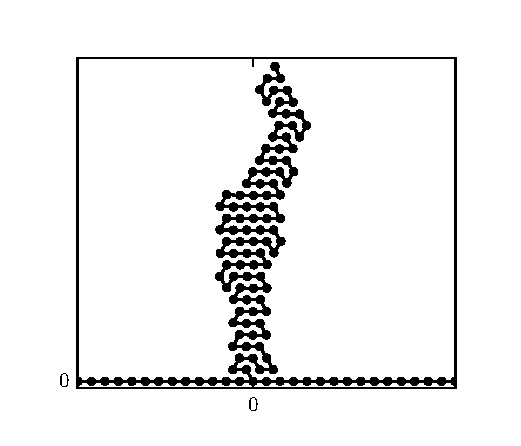
\includegraphics{./fig/ch3/fs/b0.2_eb3.eps}
			\caption{$\beta=0.2$ and $\eps_-=3$.\label{subfig:crystal1}}
		\end{subfigure}%
		~
		\begin{subfigure}{.5\textwidth}
			\centering
			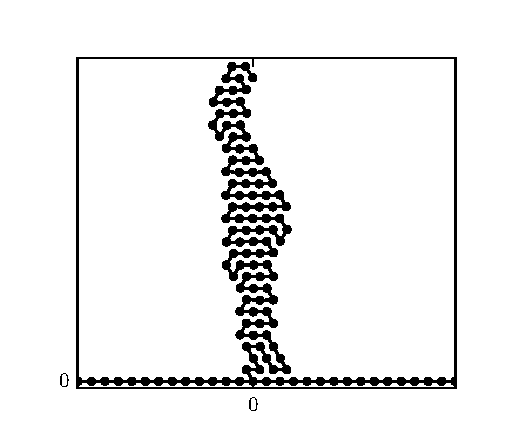
\includegraphics{./fig/ch3/fs/b0.2_eb9.eps}
			\caption{$\beta=0.2$ and $\eps_-=9$.\label{subfig:crystal2}}
		\end{subfigure}	
		\caption{Small $\beta$ of Figure~\ref{fig:fs} corresponds to fibers that crystallize with themself. Note the specific kind of crystallization of (a) and (b) as a pseudo-hexagonal chain configuration of the particles. Kinds of crystallization can be similar as with (c) and (d) but sutbly different.\label{fig:crystal}}	
	\end{figure*}

The white region of the plot consists of configurations were the fiber is either orthogonal to the bottom substrate, slanted but straight, or curved. In fact, we conjecture that a significant bend can only happen at the root, that all other particles are negligibly bent, and that if the root particle adheres to the bottom substrate then all particles will. Consider that the root particle of the fiber is nearest to the bottom substrate and will experience the strongest vdW interaction with the bottom substrate relative to any other fiber particle. If the vdW interaction causes the root particle torsional spring to bend but not buckle, then the force applied to the immediate next particle will be significantly smaller creating a negligible bend. If the vdW interaction is strong enough to cause the root particle to adhere to the bottom substrate then the torsional spring and the vdW interaction will move the next particle into an adhered state, and then the next, and so on. We observe from this argument a linear relationship between $\beta$ and $\eps_-$ at the dividing line between the white and black region. With sufficiently large $\beta$ relative to $\eps_-$ the fiber is not slanted (see Figure~\ref{subfig:erect}), and as $\beta$ decreases and $\eps_-$ increases, staying in the white region of Figure~\ref{fig:fs}, the fiber becomes more slanted (see Figure~\ref{subfig:leaning}).

They grey subregions of the plot are more complex and correspond to buckling at other particles of the fiber other than the root or fiber crystallization. Near the black region as $\eps_-$ is increased there is a gradual change from one buckle to two and so on. It appears that the particle at which buckles appear happen closer to the root with increased $\eps_-$ as well. The linear relationship between $\beta$ and $\eps_-$ is qualitative present between not only the white and black region, but the black and grey, and different grey shades. However, as $\beta$ decreases the slope increases. This trend hints that with smaller $\beta$ the fiber is more likely to crystallize. Crystallization for small $\beta$ is difficult to categorize with our adhesion heuristic, but Figure~\ref{fig:crystal} presents example crystallization configurations to help with our intuition. Most notably are configurations were the fiber can be said to be still ``standing'' as if the fiber to fiber vdW interaction has replace the torsional spring energy as a method of fiber stiffness (see Figure~\ref{subfig:hex_chain} and Figure~\ref{subfig:leaning_hex_chain}).

\section{Compression}

	\begin{table}[th]
		\rowcolors{1}{}{lightgray}
		\centering
		\caption{Reference parameters for compression.\label{table:compression_reference}}
		\begin{tabular}{lcrclcr}
			$m$ & = & 1 & \hspace{1in} & $\ell_-$ & = & 1 \\
			$n$ & = & 96 & & $\ell_+$ & = & 1 \\
			$n_+$ & = & 400 & & $\ell$ & = & 1 \\
			$n_-$ & = & 200 & & $\gamma$ & = & 100 \\
			$x^{(-)}$ & = & -100 & & $\beta$ & = & 10 \\
			$y^{(-)}$ & = & 0 & & $\eps_-$ & = & 1 \\
			$x^{(+)}$ & = & -200 & & $\eps_+$ & = & 1 \\
			$y^{(+)}$ & = & 110 & & $\eps$ & = & 1 \\
			$\delta$ & = & 0 & & $\sigma$ & = & 1
		\end{tabular}
	\end{table}
For the compression experiment a fiber is initially standing (see Figure~\ref{subfig:erect}). The primary focus is equilibrium configurations of the fiber under varying loads from the top substrate. Initially the top substrate is sufficiently far away from every particle on the fiber to prevent any vdW interaction, and because of this only loads with some nonzero positive vertical component are considered. A set of reference parameters in Table~\ref{table:compression_reference} are used in every case unless values are explicitly stated otherwise.

\subsection{Reference parameters}

	\begin{figure}[t]
		\begin{center}
			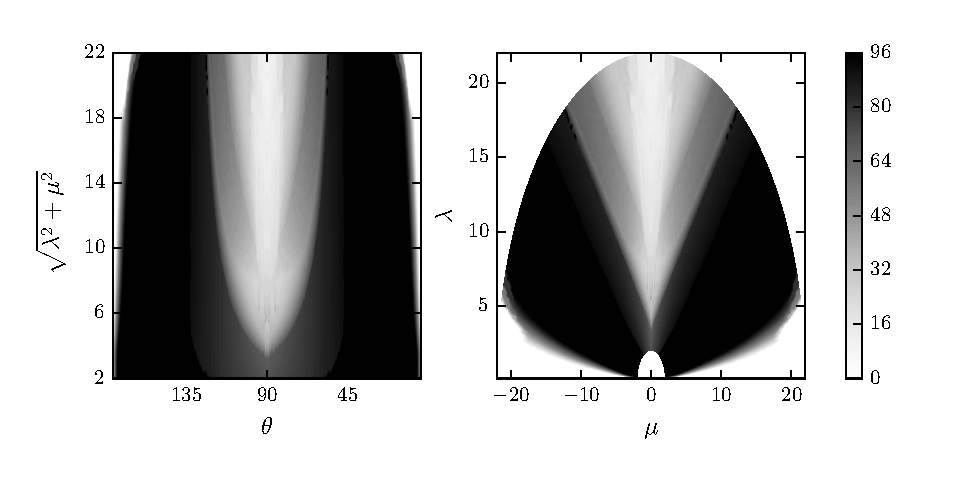
\includegraphics{./fig/ch3/push/ref/grid.eps}
		\end{center}		
		\caption{Plot of vertical component of load applied to the top substrate, $\lambda$, by the horizontal component, $\mu$, colored by adhered (fiber) particle count to the top substrate on the right. On the left is the same plot represented instead by the angle of the load by the load's magnitude colored in the same way. The black region consists of fibers that are in the \textit{flattened} configuration. There are obvious qualitative delineations of the plot by color but the categorization of the associated fiber configuration is not trivial.
		\label{fig:push:ref}}
	\end{figure}


Figure~\ref{fig:push:ref} plots the horizontal component of the load applied to the top substrate by it's vertical component colored by fiber particle adhesion to the top substrate. Analysis of contour plots of this nature will be the main focus of the results presented for the compression experiment. As with the free standing experiment, the black region of the plot corresponds to a flattened configuration as shown in Figure~\ref{subfig:flattened}. Indeed, for the contour plots of this kind throughout this section the black region will correspond to this and only this configuration. Aside from the black region there are other qualitative features of the plot: a white region, three distinct grey regions with sufficiently large magnitude of the load, small dark patches between two of those grey regions, and small grey patches in the white region for small magnitude of the load. We will explore the different regions of the plot through example.

For the darkest grey region we select $\lambda=14$ and $\mu=10.5$ as seen in Figure~\ref{subfig:flat_loop}. The configuration has one buckling point or \textit{kink}. A \textit{kink} is a buckle in a fiber that consists of relatively few particles and has sharp interior angles between bonds. This is contrast to what we consider a \textit{bend} in a fiber which consists of potentially many particles and small interior angles. For the darkest grey region we conjecture that as the angle of the load on the top substrate, $\theta$, is increased from $45$\textdegree the particle at which the kink in the fiber occurs will change to one further up the chain, thus causing less particles to be adhered.

	\begin{figure*}[h!]
		\centering
		\begin{subfigure}{.5\textwidth}
			\centering
			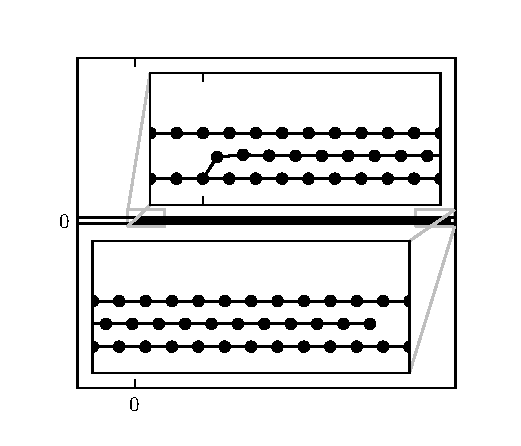
\includegraphics{./fig/ch3/push/ref/l5_m10.eps}
			\caption{$\lambda=5$ and $\mu=10$.\label{subfig:flattened}}
		\end{subfigure}%
		~
		\begin{subfigure}{.5\textwidth}
			\centering
			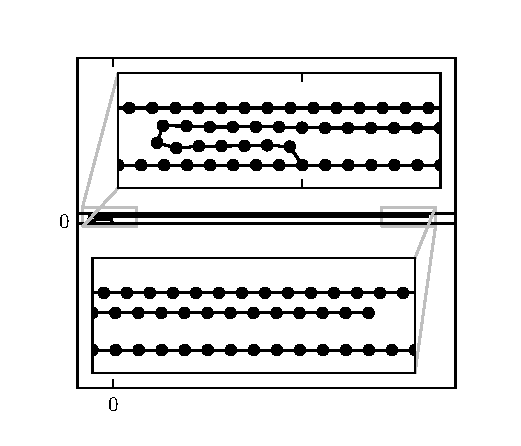
\includegraphics{./fig/ch3/push/ref/l14_m10.5.eps}
			\caption{$\lambda=14$ and $\mu=10.5$. \label{subfig:flat_loop}}
		\end{subfigure}

		\begin{subfigure}{.5\textwidth}
			\centering
			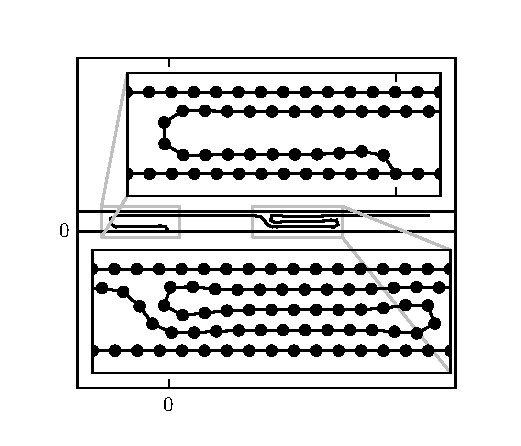
\includegraphics{./fig/ch3/push/ref/l15.5_m6.eps}
			\caption{$\lambda=15.5$ and $\mu=6$.\label{subfig:lonely_pancake}}
		\end{subfigure}%
		~
		\begin{subfigure}{.5\textwidth}
			\centering
			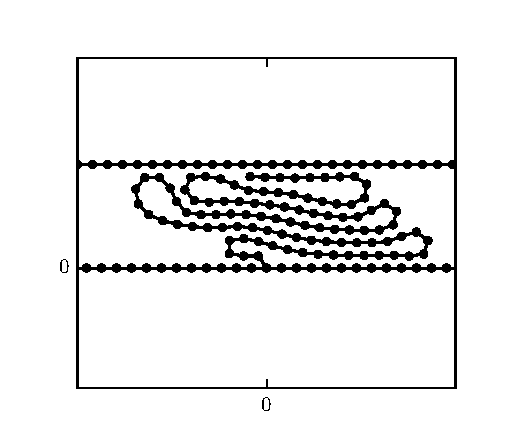
\includegraphics{./fig/ch3/push/ref/l19_m0.5.eps}
			\caption{$\lambda=19$ and $\mu=0.5$.\label{subfig:crushed}}
		\end{subfigure}
		\caption{Fiber configurations using the reference parameters in Table~\ref{table:compression_reference} with varying load. A contour plot of the adhered particle count is shown in Figure~\ref{fig:push:ref}. The black region of contour plot corresponds to (a) flattened fibers. They white region corresponds to configurations with (d) many folds. The grey region is complex and has different configurations two of which are shown in (b) and (c).\label{fig:ref_normal}}
	\end{figure*}

	\begin{figure*}[th!]
		\centering
		\begin{subfigure}{.5\textwidth}
			\centering
			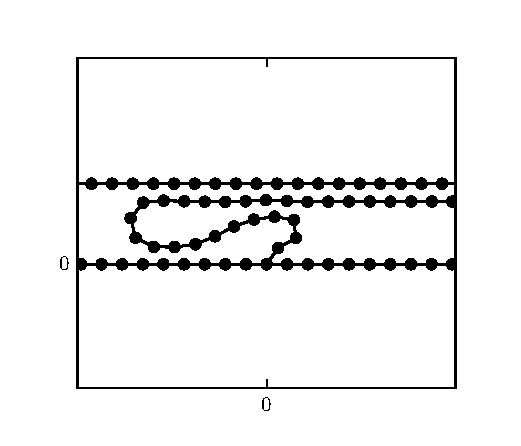
\includegraphics{./fig/ch3/push/ref/l17_m11.eps}
			\caption{$\lambda=17$ and $\mu=11$.\label{subfig:tight_loop}}
		\end{subfigure}%
		~
		\begin{subfigure}{.5\textwidth}
			\centering
			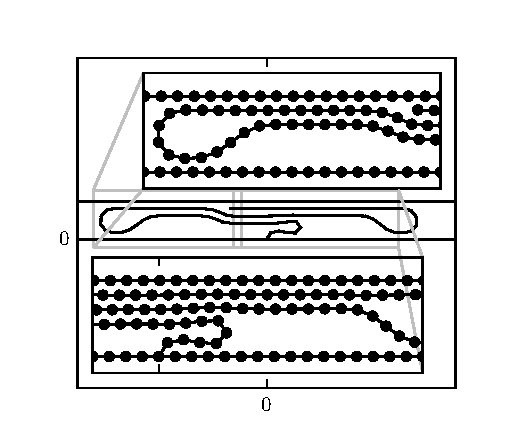
\includegraphics{./fig/ch3/push/ref/l5.9_m0.1.eps}
			\caption{$\lambda=5.9$ and $\mu=0.1$.\label{subfig:tight_hairpin}}
		\end{subfigure}
		\caption{Fiber configurations using the reference parameters in Table~\ref{table:compression_reference} with varying load. There are two locations in the contour plot of Figure~\ref{fig:push:ref} that are curious. There are patches of black between the whiter region and grey region of the plot (shown in (a)), and there are small grey pathces near the bottom of the white region (shown in (b)).\label{fig:ref_special}}
	\end{figure*}

The next darkest grey region does not have any observable difference between it and the following grey region. Configurations shown in Figure~\ref{subfig:lonely_pancake} or configurations very similar to it were observed in both regions of the plot. Although the pattern associated with the adhesion heuristic is not obvious it appears that with stronger vertical component, $\lambda$, the fiber contains more buckles (considering the same grey regions).

Figure~\ref{subfig:crushed} immediately describes the kinds of configurations that are found in the white region. The fiber is ``crushed'' underneath the load of the top substrate causing several kinks and bends. The mechanism in which some particles are able to adhere to the top substrate still while others are kept crystallized underneath the folds of the fiber itself is beyond the descriptive power of the adhesion heuristic. However, with variance in the white region in mind, equilibrium configurations are still likely to have the same ``crushed'' geometry.

Two special regions of the plot are the black patches between the darker two grey regions and the grey patches near $\theta=90$\textdegree and small magnitude of the load. We do not understand why these small regions appear. Figure~\ref{subfig:tight_loop} is an example of a configuration in the black patch region and Figure~\ref{subfig:tight_hairpin} is an example of a configuration in the grey patch region. Both configurations have bends in contrast to other configurations with similar loads with kinks.

	\begin{figure}[t]
		\begin{center}
			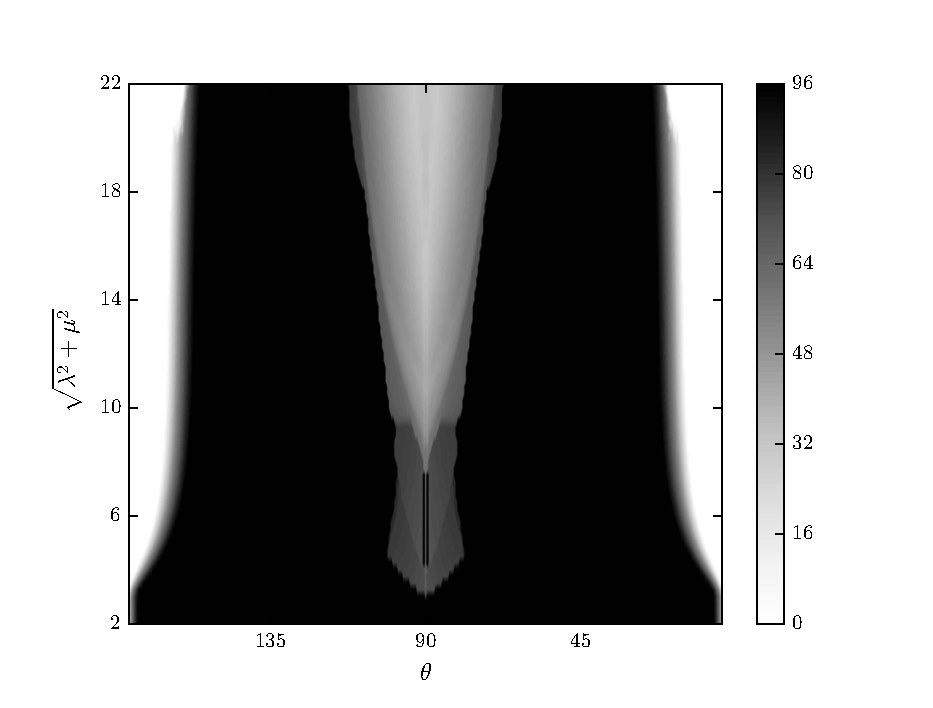
\includegraphics{./fig/ch3/push/b100/grid.eps}
		\end{center}		
		\caption{Plots of adhesive modes of a fiber under compression as in Figure~\ref{fig:push:ref}. Torsional spring strength is increased from reference parameters, $\beta=100$.
		\label{fig:push:b100}}
	\end{figure}	
	
	\begin{figure}[t]
		\begin{center}
			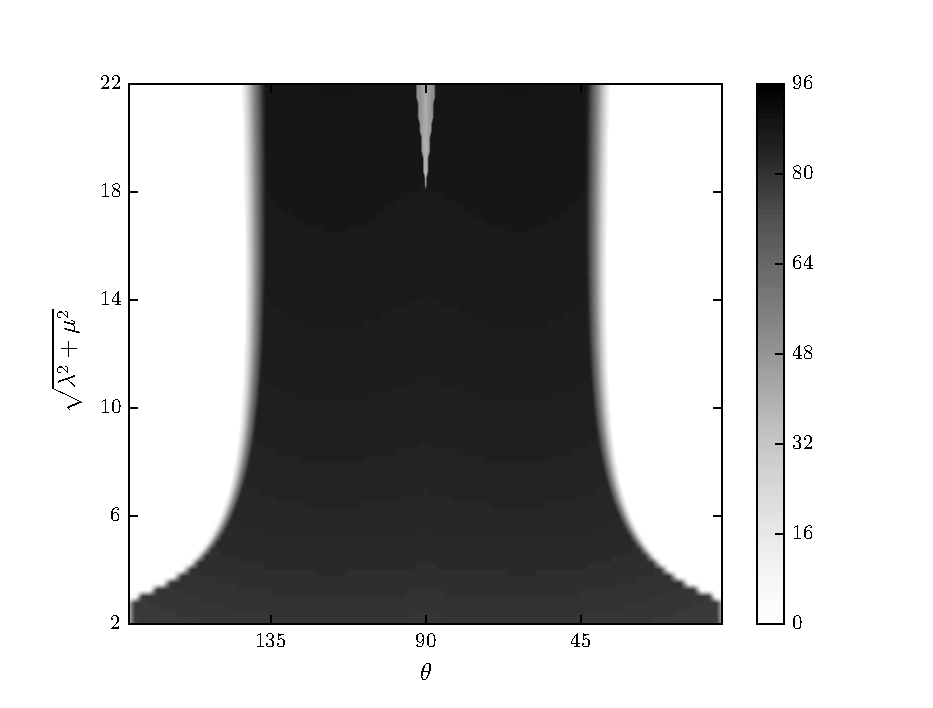
\includegraphics{./fig/ch3/push/b1000/grid.eps}
		\end{center}	
		\caption{Plots of adhesive modes of a fiber under compression as in Figure~\ref{fig:push:ref}. Torsional spring strength is increased from reference parameters, $\beta=1000$. The grey gradient from the top of the plot to the bottom immediately means that there is no strictly flattened fiber configuration.
		\label{fig:push:b1000}}
	\end{figure}
	
	\begin{figure*}
		\centering
		\begin{subfigure}{.5\textwidth}
			\centering
			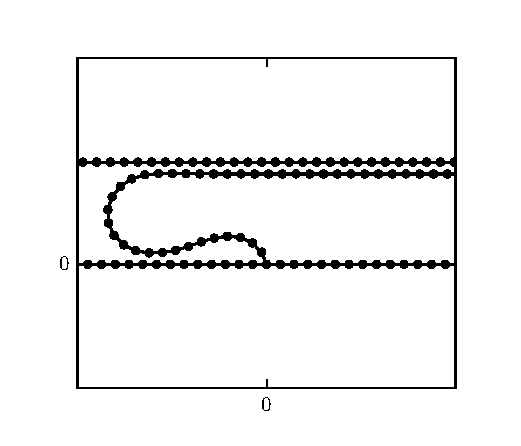
\includegraphics{./fig/ch3/push/b100/l4.6_m0.65.eps}
			\caption{$\lambda=4.6$ and $\mu=0.65$.\label{subfig:short_loop}}
		\end{subfigure}%
		~
		\begin{subfigure}{.5\textwidth}
			\centering
			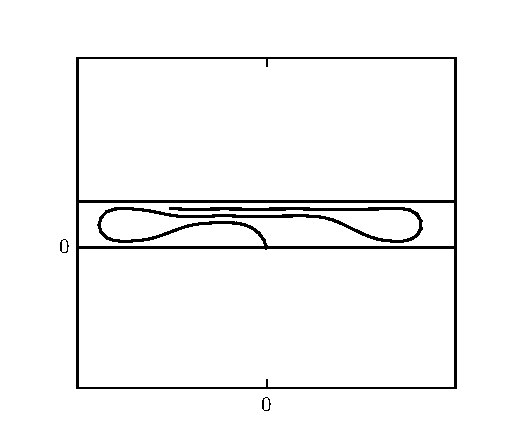
\includegraphics{./fig/ch3/push/b100/l19_m0.eps}
			\caption{$\lambda=19$ and $\mu=0$.\label{subfig:hairpin}}
		\end{subfigure}

		\begin{subfigure}{.5\textwidth}
			\centering
			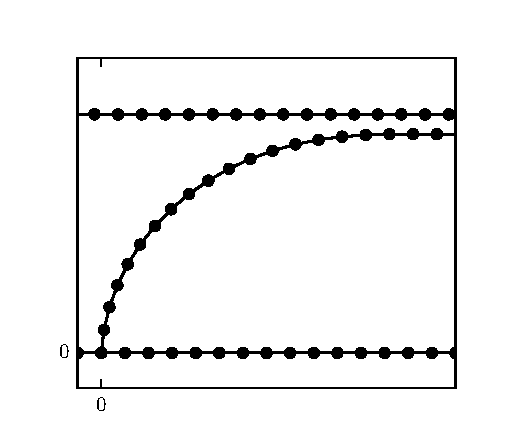
\includegraphics{./fig/ch3/push/b1000/l3_m2.eps}
			\caption{$\lambda=3$ and $\mu=2$.\label{subfig:curved}}
		\end{subfigure}%
		~	
		\begin{subfigure}{.5\textwidth}
			\centering
			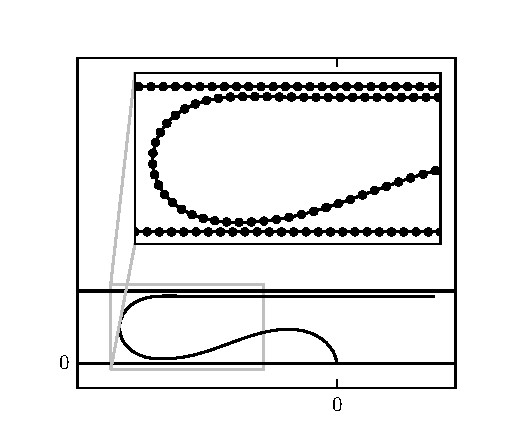
\includegraphics{./fig/ch3/push/b1000/l20_m0.eps}
			\caption{$\lambda=20$ and $\mu=0$.\label{subfig:long_loop}}
		\end{subfigure}	
		\caption{Fiber configurations using the reference parameters in Table~\ref{table:compression_reference}. Configurations (a) and (b) modify the reference paramters torsional spring string, $\beta=100$. Configurations (c) and (d) modify the same paramter, $\beta=1000$. From all configurations we note that an increase in $\beta$ correspondes to bends consisting of many particles instead of kinks consisting of few particles.\label{fig:bending_fiber}}	
	\end{figure*}

\subsection{Varying $\beta$}

The strength of the torsional spring strength, $\beta$, was shown as vitally important to a fiber moving to a flattened configuration or a standing one in Figure~\ref{fig:fs}. For the reference parameters in Table~\ref{table:compression_reference} $\beta$ is strong enough to stand freely. However, we are interested in significant modifications of the reference parameters by at least one order of magnitude. Decreasing the reference value of $\beta$ by an order of magnitude would make it too small for the fiber to stand freely. Because of this we only increase $\beta$.

Increasing $\beta$ by an order of magnitude such that $\beta=100$ significantly alters the picture from before. Shown in Figure~\ref{fig:push:b100} the black region of the plot is larger and grey and white regions have different shape. The difference in configurations for each region has much to do with precisely how many particles are part of a bend or if there is more than one bend. We present two examples: Figure~\ref{subfig:short_loop} corresponds to the black line inside the darker grey region, and Figure~\ref{subfig:hairpin} corresponds to $\theta=90$\textdegree with large magnitude.

The grey region of the contour plot is a similar configuration in Figure~\ref{subfig:short_loop} with the exception that more of the fiber is folded underneath itself causing a wave-like curve. The white regions also are similar to the example given in Figure~\ref{subfig:hairpin}. Even though there is variability in the heuristic it is because small numbers of particles are part of the curve of bends in the fiber instead of the adhered particles. This is the same idea shown in Figure~\ref{fig:push:ref} were slightly lighter portions of grey regions were because of configurations with a few particles being before instead of after the kink(s).

Increasing $\beta$ by another order of magnitude, $\beta=1000$, again significantly alters the picture. Figure~\ref{fig:push:b1000} shows the contour plot with this modification. Most notably is the loss of a black region, and a significantly smaller white region. The gradient of the grey region is represented in it's entirety with Figure~\ref{subfig:curved}. Any configuration in the grey region is only a fiber with a gradual bend from the root to the first adhered particle on the top substrate. This configuration is novel to $\beta=1000$ for the values we presented. The white region in contrast is similar to the same kind of configurations seen in the grey regions of $\beta=100$ with the exception of even more particles being in the bend (see Figure~\ref{subfig:long_loop}).

	\begin{figure}[t]
		\begin{center}
			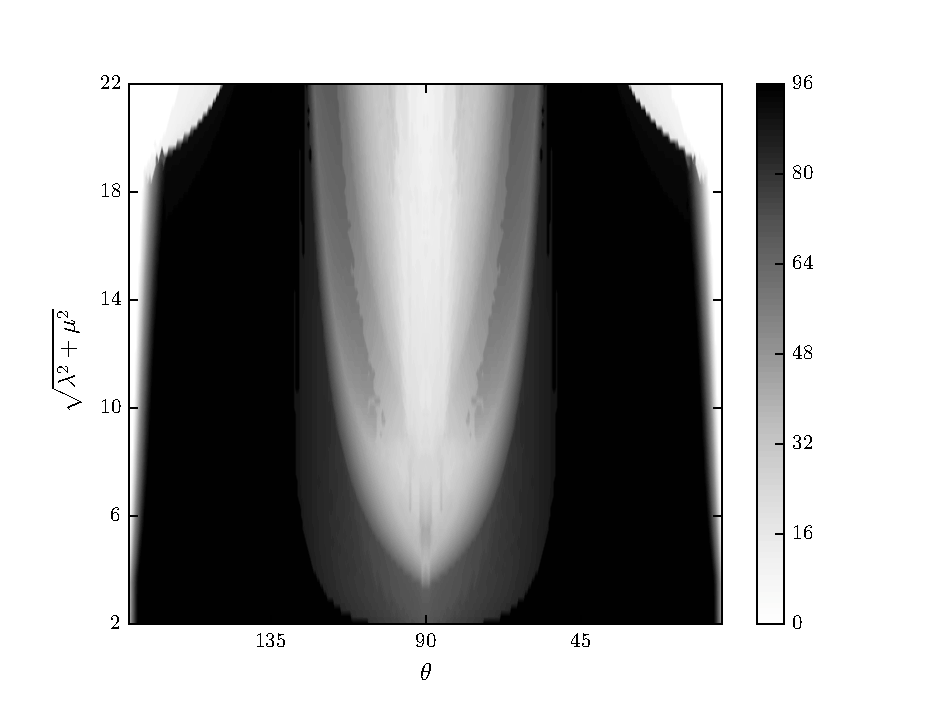
\includegraphics{./fig/ch3/push/eb0.1/grid.eps}
		\end{center}		
		\caption{Plots of adhesive modes of a fiber under compression as in Figure~\ref{fig:push:ref}. VdW interaction strength of the bottom substrate is weakened, $\eps_-=0.1$.
		\label{fig:push:eb0.1}}
	\end{figure}	

	\begin{figure}[t]
		\begin{center}
			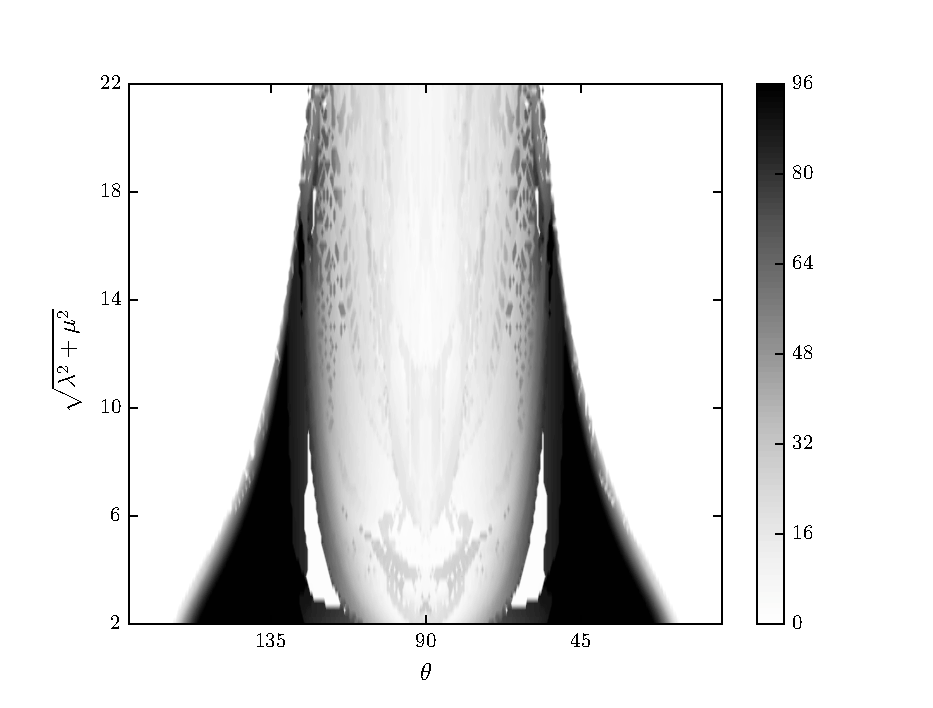
\includegraphics{./fig/ch3/push/et0.1/grid.eps}
		\end{center}		
		\caption{Plots of adhesive modes of a fiber under compression as in Figure~\ref{fig:push:ref}. VdW interaction strength of the top substrate is weakened, $\eps_+=0.1$. We note the dramatic change between this plot and Figure~\ref{fig:push:eb0.1} as they both are a weakening in vdW interaction by one order of magnitude.
		\label{fig:push:et0.1}}
	\end{figure}

	\begin{figure}[t]
		\begin{center}
			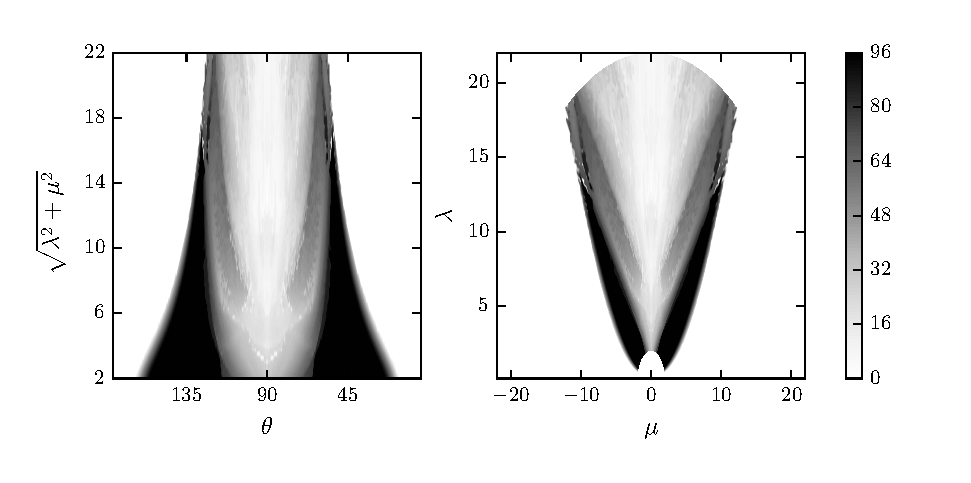
\includegraphics{./fig/ch3/push/eb0.1_et0.1/grid.eps}
		\end{center}		
		\caption{Plots of adhesive modes of a fiber under compression as in Figure~\ref{fig:push:ref}. VdW interaction strength of the top and bottom substrate is weakened, $\eps_+=0.1$ and $\eps_-=0.1$.
		\label{fig:push:eb0.1_et0.1}}
	\end{figure}	

	\begin{figure*}
		\centering
		\begin{subfigure}{.5\textwidth}
			\centering
			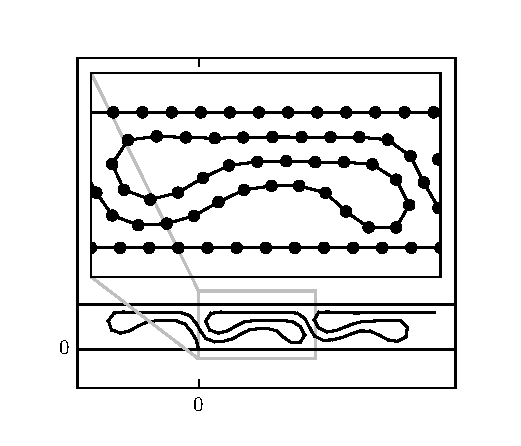
\includegraphics{./fig/ch3/push/eb0.1/l20.5_m3.5.eps}
			\caption{$\lambda=20.5$ and $\mu=3.5$.\label{subfig:multi_bridge}}
		\end{subfigure}%
		~
		\begin{subfigure}{.5\textwidth}
			\centering
			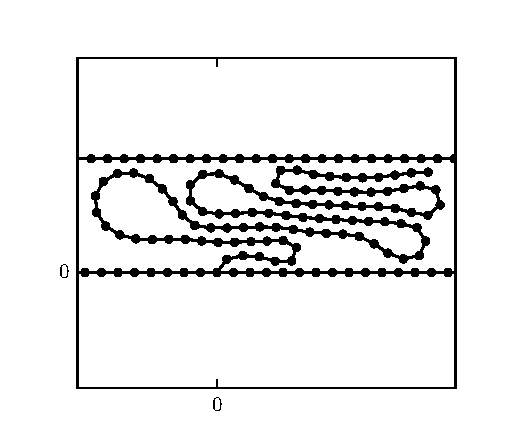
\includegraphics{./fig/ch3/push/eb0.1_et0.1/l20_m2.eps}
			\caption{$\lambda=20$ and $\mu=2$.\label{subfig:slant_crushed}}
		\end{subfigure}

		\begin{subfigure}{.5\textwidth}
			\centering
			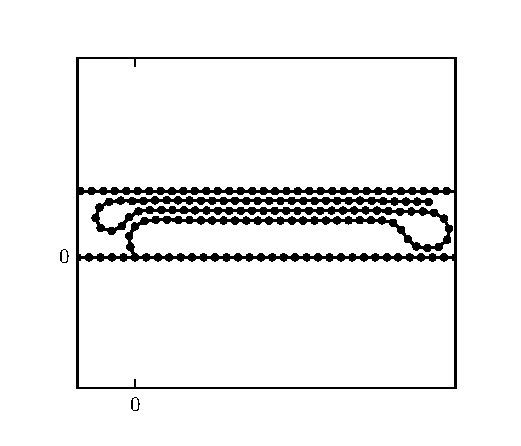
\includegraphics{./fig/ch3/push/et0.1/l4.5_m1.eps}
			\caption{$\lambda=4.5$ and $\mu=1$.\label{subfig:bridge}}
		\end{subfigure}%
		~
		\begin{subfigure}{.5\textwidth}
			\centering
			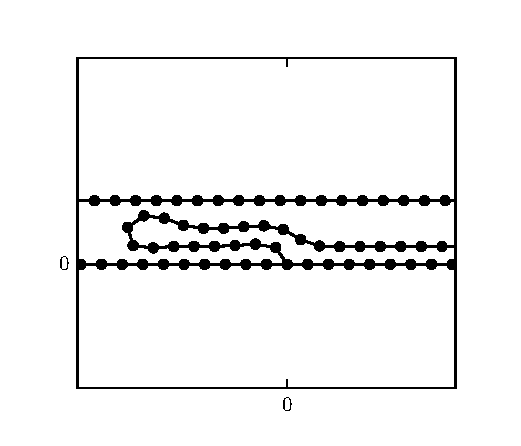
\includegraphics{./fig/ch3/push/et0.1/l6_m4.eps}
			\caption{$\lambda=6$ and $\mu=4$\label{subfig:hump}}
		\end{subfigure}	
		\caption{Fiber configurations using the reference parameters in Table~\ref{table:compression_reference}. Configuration (a) modifies the reference paramters bottom substrate vdW interaction strength, $\eps_-=0.1$. Configuration (b) modifies the reference paramters bottom and top substrate vdW interaction strength, $\eps_-=0.1$ and $\eps_+=0.1$. Configurations (c) and (d) modify the reference parameters top substrate vdW interaction strength, $\eps_+=1$.\label{fig:vdw_crushed}}	
	\end{figure*}

\subsection{Varying $\eps_-$ and $\eps_+$} \label{subsection:push:eps}

Another method of allowing a fiber to stand instead of move to a flattened configuration is to decrease the vdW interaction strengths. Namely, we are interested in decreasing the vdW interaction strengths of both substrates, first independently and then together.

As a fiber is being compressed by the top substrate, it either began the process of adhering to the bottom substrate before the top substrate reaches it, or stands and is compressed strictly by the top substrate. For the reference parameters the fiber will begin to collapse on it's on, however not to a flattened configuration. Decreasing vdW interaction strength of the bottom substrate, $\eps_-=0.1$, will cause the fiber to be free standing. This modification means that the top substrate is the principal influence over how the fiber compresses, but after the fiber has been compressed the bottom substrate can stiffen the fiber's configuration. Figure~\ref{fig:push:eb0.1} shows the contour plot with this modification. Although there are noticeable differences the picture is qualitatively similar to the reference parameters picture, Figure~\ref{fig:push:ref}.

In contrast, when we decrease vdW interaction strength of the top substrate, $\eps_+=0.1$, the picture becomes significantly more complex (see Figure~\ref{fig:push:et0.1}). Previously we partitioned contour plots into regions using the adhesion heuristic as a guide. However, when we decrease vdW interaction strength the complexity in configurations becomes difficult to manage. Because of this difficulty we focus on specific features we can speak to, the overall comparison, and provide example configurations to give an intuition of the plots. In Figure~\ref{fig:push:et0.1} we have a white region for small magnitude of the load which corresponds to a ``hump'' configuration of the fiber (see Figure~\ref{subfig:hump}). As discussed before, because $\beta$ and $\eps_-$ are equal to the reference parameters the fiber will immediately begin to adhere to the bottom substrate. The top substrate vdW interaction strength is weaker which relaxes the constraints on the fiber both while it is being compressed and after it has been compressed. This allows for a kink to form near the root and for the fiber to completely adhere to the bottom substrate.

Decreasing vdW interaction strengths of both substrates to $0.1$ is shown in Figure~\ref{fig:push:eb0.1_et0.1}. With these modifications the primary modes of buckling involve parts of the fiber crystallizing. The grey region of the plot is similar to configurations shown in the reference parameters, specifically Figure~\ref{subfig:lonely_pancake}. The white region is also similar, consisting of ``crushed'' fiber configurations.

Example configurations for decreased vdW interaction strength are shown in Figure~\ref{fig:vdw_crushed}. These examples demonstrate some of the kinds of buckling that are exhibited but large categorizations of configurations as mentioned before difficult. With previous examples it was not wrong to assume, at least locally to the region in discussion, that the configurations were similar to the examples presented, but for these examples that is not necessarily true.
	
	\begin{figure}[t]
		\begin{center}
			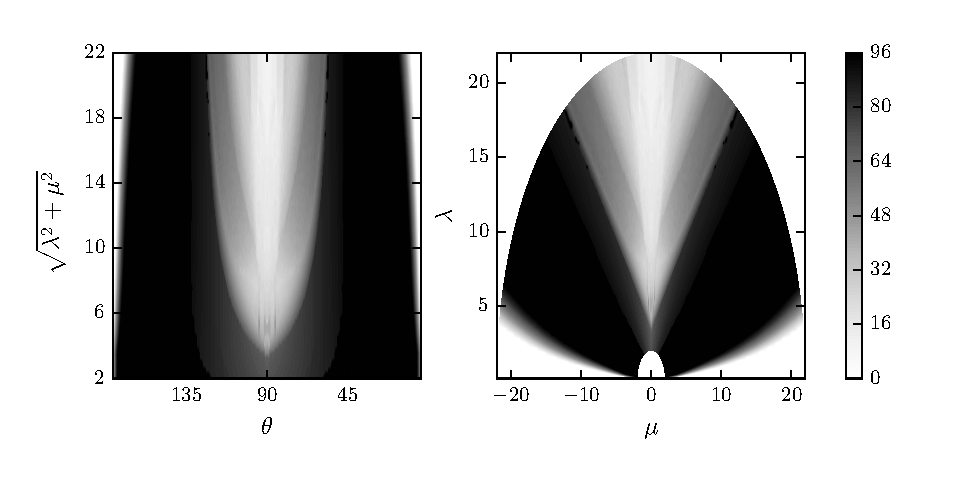
\includegraphics{./fig/ch3/push/g1000/grid.eps}
		\end{center}		
		\caption{Plots of adhesive modes of a fiber under compression as in Figure~\ref{fig:push:ref}. Extensible spring constant is increased, $\gamma=1000$.
		\label{fig:push:g1000}}
	\end{figure}	

\subsection{Varying $\gamma$}

We modify the extensible spring constant to ensure that our reference selecton, $\gamma=100$, is sufficiently large so that the fiber is sufficiently stiff. Figure~\ref{fig:push:g1000} for $\gamma=1000$ shows a contour plot similar to the reference plot (see Figure~\ref{fig:push:ref}). There are no qualitative differences between them which suggests that our selection of $\gamma$ is adequate.

	\begin{figure}[t]
		\begin{center}
			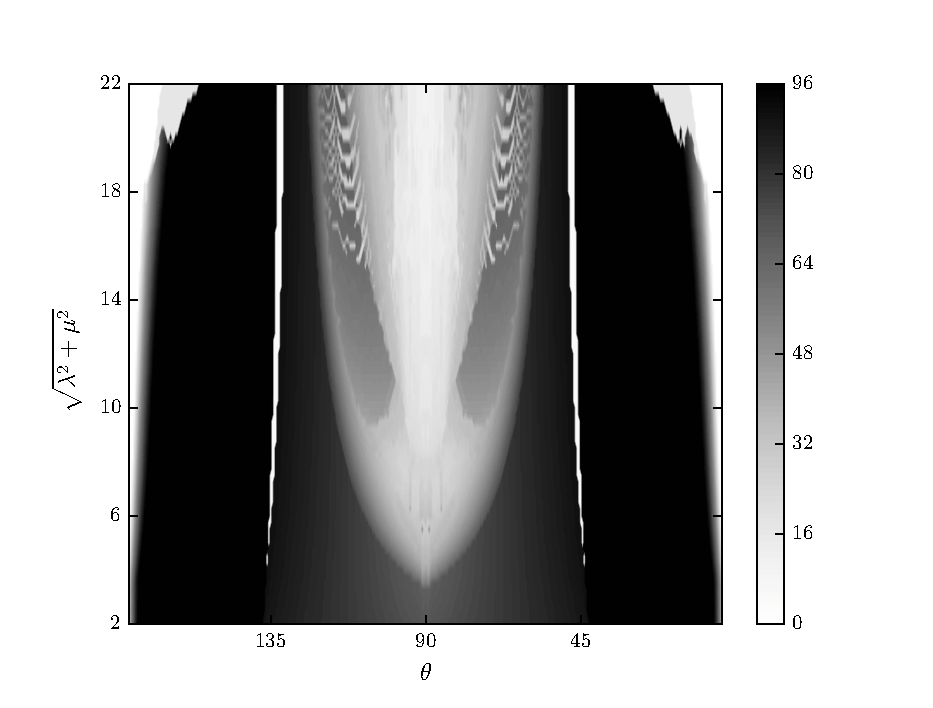
\includegraphics{./fig/ch3/push/p1/grid.eps}
		\end{center}		
		\caption{Plots of adhesive modes of a fiber under compression as in Figure~\ref{fig:push:ref}. The bottom substrate is replaced with a continuum of particles, that is the vdW interaction is integrated over the a bottom substrate of infinite length. The strength of the continuum vdW interaction is $p=1$.
		\label{fig:push:p1}}
	\end{figure}

\subsection{Bottom substrate with uniform potential} \label{section:compression:pressure}

A tangential curiosity is how the system behaves when the bottom substrate is a uniform potential instead of particle-particle potentials. We assume the bottom substrate is composed of infinitely many particles by integrating the Lennard-Jones potential. Every particle of the fiber interacts with the bottom substrate to this new uniform potential instead of a particle-particle potential.

Using the adhesion heuristic we see a similar picture to the reference parameters for the uniform potential (see Figure~\ref{fig:push:p1}). There are differences, most notably the white region of the plot between the black and dark grey regions. This region is the same kind of ``hump'' configuration we've seen before in Figure~\ref{subfig:hump}. Overall, we conjecture from both plots, Figure~\ref{fig:push:ref} and Figure~\ref{fig:push:p1}, that the different potentials give the same general behavior for the equilibrium configurations of the fiber, with some exceptions. This is however a limited comparison and those exceptions are not minor.

\section{Detachment} \label{ch:detachment}

In both the free standing and compression experiments we focused on a range of values of interest and presented a contour plot of the space using a heuristic for adhesion. With the detachment experiment we can explore the parameter space more intelligently. Instead of an exhaustive approach we assume that there is a critical magnitude of the load on the top substrate such that it will ``detach'' from the fiber. The top substrate is said to \textit{detach} from the fiber at the point in time when no particles of the fiber are adhered to the top substrate. If there is in fact a critical magnitude of the load for a given angle of the load then we can heuristically pick a sufficiently large magnitude such that the top substrate does detach and then bisect between that value and $0$. Note that the existence of a critical magnitude is not true in general and we will discuss such cases when they occur.

All simulations for the detachment experiment begin with the system in a flattened configuration (see Figure~\ref{subfig:flattened}). Although there are several compressed configurations from the previous experiment we focus on only the flattened configuration in this work.

	\begin{table}
		\rowcolors{1}{}{lightgray}
		\centering
		\caption{Reference parameters for the detachment experiment. \label{table:detachment_reference}}
		\begin{tabular}{lcrclcr}
			$m$ & = & 1 & \hspace{1in} & $\ell_-$ & = & 1 \\
			$n$ & = & 96 & & $\ell_+$ & = & 1 \\
			$n_+$ & = & 300 & & $\ell$ & = & 1 \\
			$n_-$ & = & 300 & & $\gamma$ & = & 100 \\
			$x^{(-)}$ & = & -150 & & $\beta$ & = & 1 \\
			$y^{(-)}$ & = & 0 & & $\eps^-$ & = & 1 \\
			$x^{(+)}$ & = & -150 & & $\eps^+$ & = & 1 \\
			$y^{(+)}$ & $\approx$ & 1.72741 & & $\eps$ & = & 1 \\
			$\delta$ & = & 0 & & $\sigma$ & = & 1
		\end{tabular}
	\end{table}
	
	\begin{figure}
		\begin{center}
			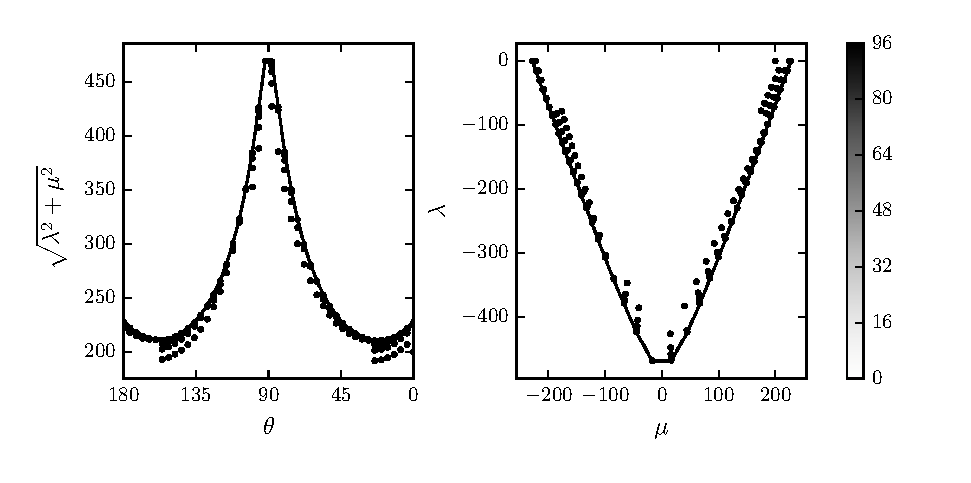
\includegraphics{./fig/ch3/pull/ref/grid.eps}
		\end{center}		
		\caption{The left is a plot of minimum critical load for the top substrate to detach from the fiber as function of the angle of the load. The right is the same plot in terms of the horizontal and vertical component of the load on the top substrate. For any given angle the critical load is only approximate, thus there are actually two lines drawn, one solid black representing the smallest detachment load, and a dashed line beneath it representing the largest adhesive load. Each circle represents a specific simulation.
		\label{fig:pull:ref}}
	\end{figure}

\subsection{Reference parameters}

As with the compression experiment we have a set of selected reference parameters in Table~\ref{table:detachment_reference}. Figure~\ref{fig:pull:ref} shows the critical magnitude for detachment of the load as a function of the angle of the load on the left, and the same line plotted via the components of the load on the right. There is a linear interpolation between every $4$th angle in the plot which makes determining maxima and minima to high absolute accuracy difficult but we are more interested in qualitative trends anyway. Every circle of the plot is a simulation for some specific value of $\lambda$ and $\mu$, and the color of the circle is the value of the adhesion metric between the fiber and the top substrate. All plots of the critical magnitude for detachment will follow these patterns.

Unlike the compression experiment, the detachment experiments do not yield as interesting equilibrium configurations. Above the critical magnitude in every case is a return to the free standing experiment with a different initial condition, and although that is interesting in it's own way the equilibrium configurations of those cases are not the focus of this experiment. Thus we ignore any simulations and configurations that happen above the critical magnitude. For the reference parameters, equilibrium configurations below the critical magnitude are all identical, they are the flattened configuration. Clearly the adhesion heuristic that has given us some success is not helpful in this case. In order to understand the picture then we turn to discussing the dynamics of the system under a detaching magnitude.

In the range $0 \leq \theta < 45$ the top substrate detaches from the fiber by sliding. The top substrate is said to ``slide'' if the particles on the top substrate shift from equilibrium with a collection of fiber particles to an equilibrium position with different collection of fiber particles in a finite amount of time. We conjecture there is a minimum in this range of $\theta$ values because there is an optimal angle of the load to maximize the number of particles are ``skipped'' when the top substrate slides across the fiber. As the angle of the load increases the effective horizontal distance traveled is reduced instead of improved.

Considering the range $45 \leq \theta < 90$ the top substrate continues the sliding mode of detachment up until what is assumed to be a critical angle where the effective horizontal displacement of a single particle on the top substrate is too small to slide over a single particle of the fiber. At this critical angle the mode of detachment changes from sliding to brute force. The top substrate is said to detach from the fiber via ``brute force'' if the critical magnitude of the load must be large enough to break every vdW interaction between the fiber and the top substrate simultaneously.

The range $90 \leq \theta \leq 180$ is similar. There is a critical angle of the load such that the top substrate changes from detaching from the fiber via brute force to detaching from the fiber by sliding, and there is a minimum angle of the load such that the displacement of a given particle on the top substrate is maximized during sliding. However, the way in which sliding occurs is subtly different. There is an observable asymmetry in the plot which is not fully understood. One explanation is that if the top substrate pulls against the direction that the fiber has been flattened (in this case to the right) then the torsional spring energy will push a particle of the fiber up into the top substrate repelling it from the fiber and thus making it easier to slide.

The plot on the right of Figure~\ref{fig:push:ref} tells the same story from a different perspective. With it we can see that the critical load is a linear relationship between the components of the load $\lambda$ and $\mu$ on either side of$\theta=90$\textdegree . 

	\begin{figure}[t]
		\begin{center}
			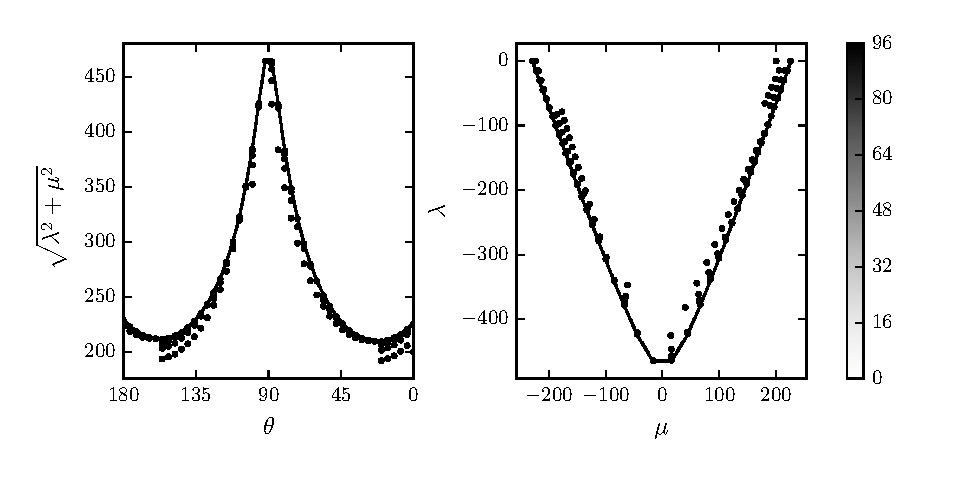
\includegraphics{./fig/ch3/pull/b10/grid.eps}
		\end{center}		
		\caption{Plot of the minimum critical magnitude for detachment as in Figure~\ref{fig:pull:ref}. The torsional spring strength is increased, $\beta=10$, from the reference parameters in Table~\ref{table:detachment_reference}.
		\label{fig:pull:b10}}
	\end{figure}
	
	\begin{figure}[t]
		\begin{center}
			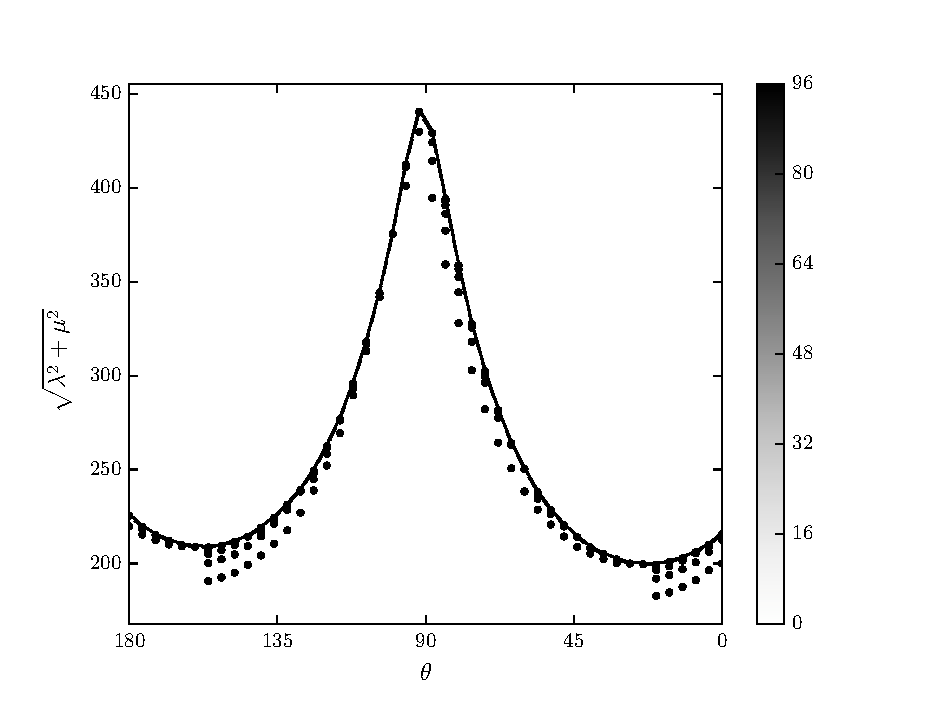
\includegraphics{./fig/ch3/pull/b100/grid.eps}
		\end{center}		
		\caption{Plot of the minimum critical magnitude for detachment as in Figure~\ref{fig:pull:ref}. The torsional spring strength is increased, $\beta=100$.
		\label{fig:pull:b100}}
	\end{figure}
	
\subsection{Varying $\beta$}

For the compression experiment $\beta$ was already sufficiently large for a fiber to stand freely. In the case of the detachment experiment $\beta=1$ is a magnitude lower and the fiber will not be able to stand freely. Like before, with the same reasoning, we focus only on increasing $\beta$.

With increased $\beta$ the story does not signficantly change. Figure~\ref{fig:pull:b10} and Figure~\ref{fig:pull:b100} show plots that are similar in general shape to the reference parameters. When the dynamics of a detachment are observed they are also very similar to the reference parameters. However, the values of extrema are different with larger $\beta$. The local minimum of the critical detachment load to the left of the maximum value is larger as $\beta$ increases. In contrast, the minimum value to the right of the maximum value of smaller as $\beta$ increases. This means the asymmetry in the plot is more exaggerated with larger $\beta$. This observation is consistent with the given explanation for the asymmetry being related to torsional springs near the root particle of the fiber. Lastly, the maximum critical magnitude decreases as $\beta$ increases.

	\begin{figure}
		\begin{center}
			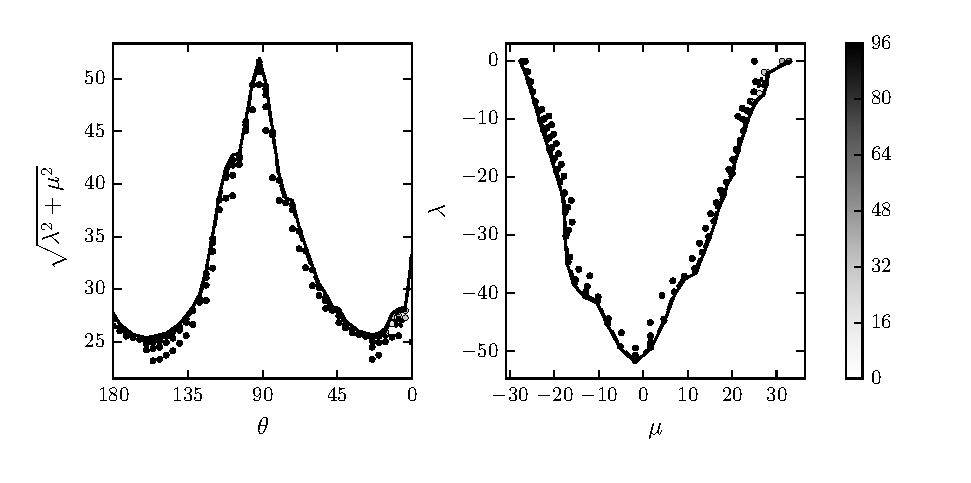
\includegraphics{./fig/ch3/pull/eb0.1/grid.eps}
		\end{center}		
		\caption{Plot of the minimum critical magnitude for detachment as in Figure~\ref{fig:pull:ref}. The strength of the vdW interaction for the bottom substrate is decreased, $\eps_-=0.1$. In both plots there is a black star marker which corresponds to a detachment magnitude that happens below what we consider the critical magnitude.
		\label{fig:pull:eb0.1}}
	\end{figure}

	\begin{figure}
		\begin{center}
			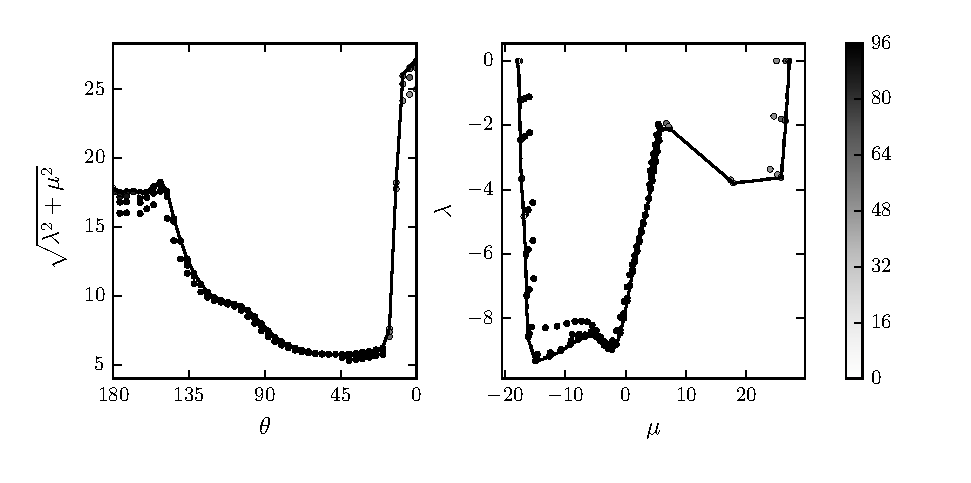
\includegraphics{./fig/ch3/pull/eb0.01/grid.eps}
		\end{center}		
		\caption{Plot of the minimum critical magnitude for detachment as in Figure~\ref{fig:pull:ref}. The strength of the vdW interaction for the bottom substrate is decreased, $\eps_-=0.01$. 
		\label{fig:pull:eb0.01}}
	\end{figure}
	
	\begin{figure}
		\begin{center}
			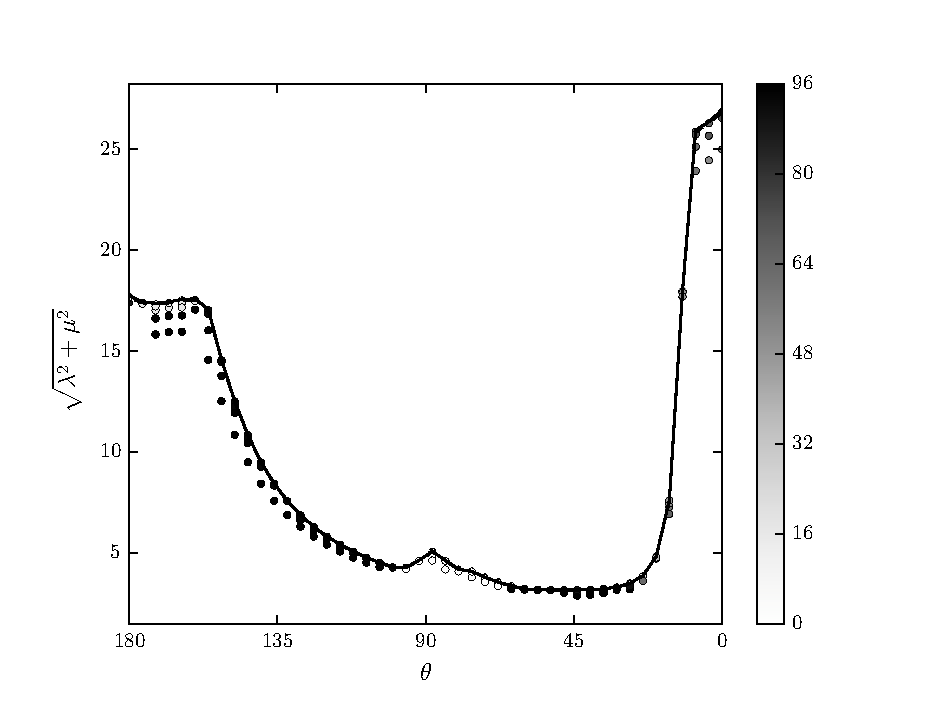
\includegraphics{./fig/ch3/pull/eb0/grid.eps}
		\end{center}		
		\caption{Plot of the minimum critical magnitude for detachment as in Figure~\ref{fig:pull:ref}. The strength of the vdW interaction for the bottom substrate is removed, $\eps_-=0$. Note that simulation circles that are white are not the same as star markers representing isolated detachments.
		\label{fig:pull:eb0}}
	\end{figure}
	
	\begin{figure}
		\begin{center}
			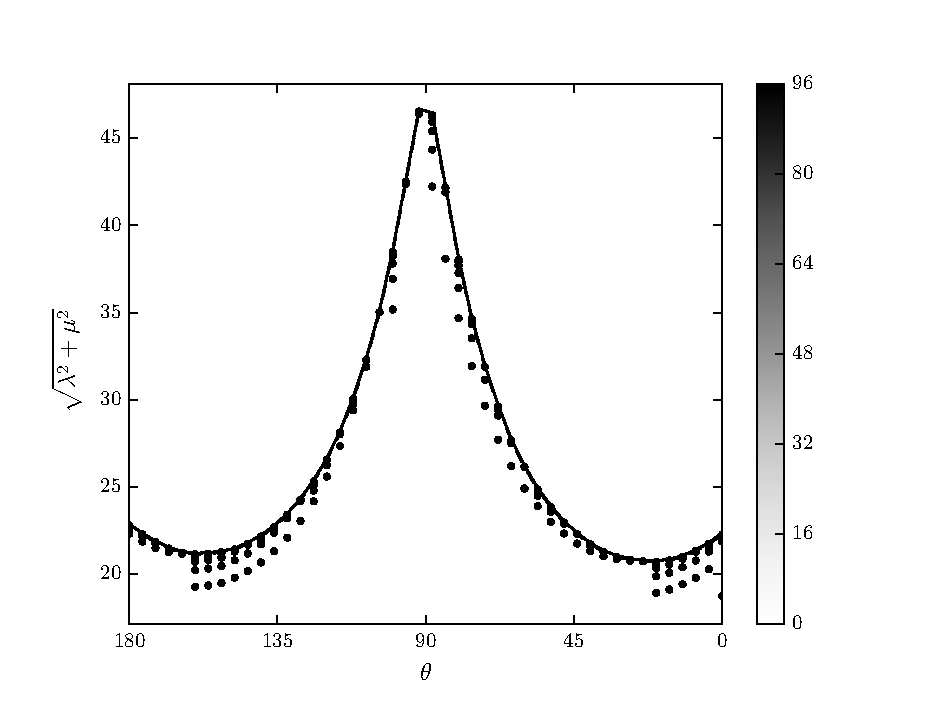
\includegraphics{./fig/ch3/pull/eb0.1_et0.1/grid.eps}
		\end{center}		
		\caption{Plot of the minimum critical magnitude for detachment as in Figure~\ref{fig:pull:ref}. The strength of the vdW interaction for the bottom and top substrate are decreased, $\eps_-=0.1$ and $\eps_+=0.1$.
		\label{fig:pull:eb0.1_et0.1}}
	\end{figure}
	
	\begin{figure}
		\begin{center}
			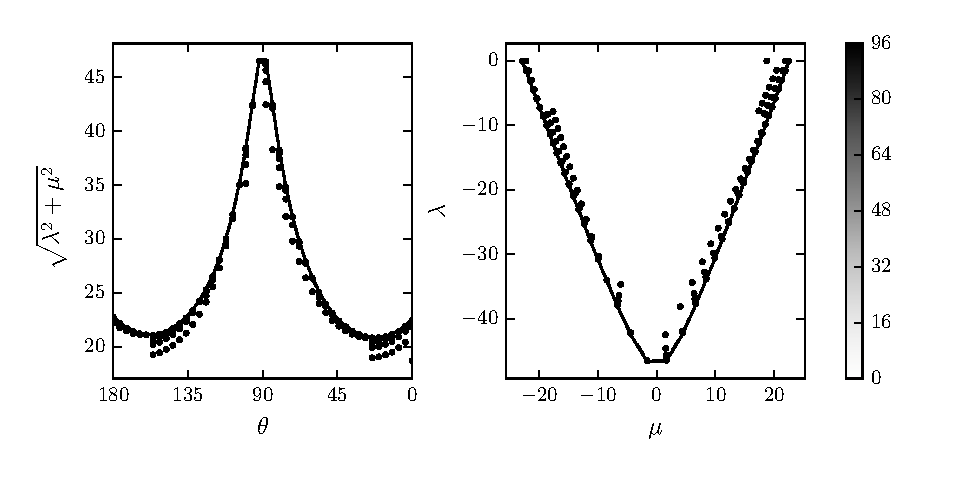
\includegraphics{./fig/ch3/pull/eb0.1_et0.1_e0.1/grid.eps}
		\end{center}		
		\caption{Plot of the minimum critical magnitude for detachment as in Figure~\ref{fig:pull:ref}. The strength of the vdW interaction for all particles are decreased, $\eps_-=0.1$, $\eps_+=0.1$, and $\eps=0.1$.
		\label{fig:pull:eb0.1_et0.1_e0.1}}
	\end{figure}
	
	\begin{figure}
		\begin{center}
			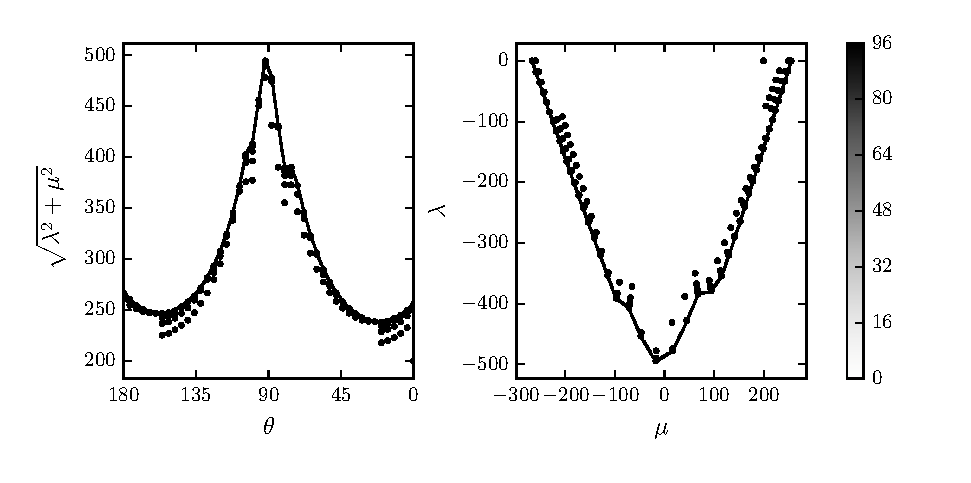
\includegraphics{./fig/ch3/pull/et10/grid.eps}
		\end{center}		
		\caption{Plot of the minimum critical magnitude for detachment as in Figure~\ref{fig:pull:ref}. The strength of the vdW interaction for the top substrate is increased, $\eps_+=10$.
		\label{fig:pull:et10}}
	\end{figure}

\subsection{Varying $\eps^-$, $\eps^+$, and $\eps$} \label{section:detachment:eps}

Varying vdW interaction strengths has the most significant effect on the results of the detachment experiment that we have observed. First, we consider decreasing $\eps_-$ and $\eps_+$ to $0.1$ and related all three vdW interactions, $\eps_- = \eps_+ = \eps = 0.1$. Second, we consider the case were only $\eps_-=0.1$ and the case where only $\eps_+=10$. Lastly, we consider decreasing $\eps_-$ further, exploring both $\eps_-=0.01$ and $\eps_-=0$.

For $\eps_- = \eps_+ = 0.1$ the critical magnitude for detachment is decreased for all angles of the load by approximately an order of magnitude. Figure~\ref{fig:push:eb0.1_et0.1} demonstrates the linear relationship between the critical detachment load and vdW uniform decrease in the substrate interaction strengths. However, the modes of detachment are significantly different. 


For the same reason we only increase $\beta$, here we only decrease the vdW interaction strengths. Our first interest is in decreasing $\eps^-$ only. Here we notice an exception in the assumptions we've used so far. An \textit{isolated detachment} is a load that will cause the upper substrate to detach from the fiber even though with a small increase in magnitude the substrate would stay adhered. The reasons for this have much to do with the propagating wave and how the upper substrate's particles align with the fiber's particles. Even one reduction in order of magnitude of $\eps^-$ has a significant qualitative effect (see Figure~\ref{fig:PullGrid:eb0.1}). The magnitude required for the upper substrate to detach is significantly less for every angle. Moreover, although the general symmetry survives to a certain point there are significantly more asymmetries. As $\eps^-$ is reduced by another order of magnitude the picture changes entirely as we can see from Figure~\ref{fig:PullGrid:eb0.01}. With the adhesion between the fiber and the bottom substrate so significantly weakened the reinforcement of the flattened state is removed and allows for the upper substrate to zip free of the fiber one vdW bond at a time. Thus, the initial resistance in moving the root and causing a propagating wave is no longer the primary method of detachment and becomes the greatest hindrance instead. When $\eps^-$ is reduced to the point of vanishing this zipping around no shear component becomes more obvious as magnitude just slightly below the minimum has only one particle adhered to the upper substrate (see Figure~\ref{fig:PullGrid:eb0}). It would seem then that zipping is an efficient enough method of detachment that it is easier to zip free of a bond than it is to break one. The resistance when there is primarily only a shear component again has the same difficulty as before.

In Figure~\ref{fig:PullGrid:eb0.1_et0.1} we reduce both $\eps^-$, and $\eps^+$ by an order of magnitude. In comparison to the reference parameters the major difference is in the required magnitude to detach. This would seem like the obvious consequence as vdW bonds are the only reason for attachment. In Figure~\ref{fig:PullGrid:eb0.1_et0.1_e0.1} $\eps$ is also reduced by an order of magnitude, but there is no qualitative difference between the two. We also increase just $\eps^+$ in one case (see Figure~\ref{fig:PullGrid:et10}). We can see from the figure that it is most directly comparable to Figure~\ref{fig:PullGrid:eb0.1}.

	\begin{figure}
		\begin{center}
			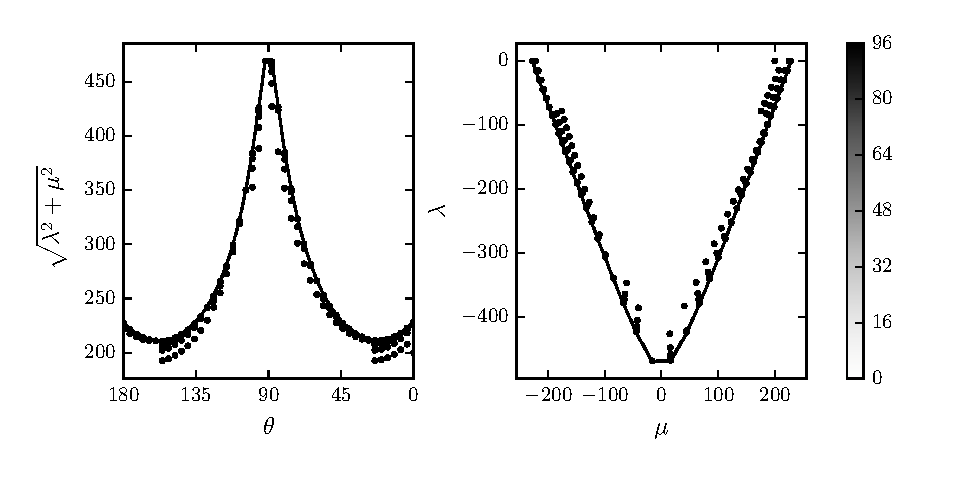
\includegraphics{./fig/ch3/pull/g1000/grid.eps}
		\end{center}		
		\caption{Plot of the minimum critical magnitude for detachment as in Figure~\ref{fig:pull:ref}. The extensible spring constant is increased, $\gamma=1000$.
		\label{fig:pull:g1000}}
	\end{figure}

\subsection{Varying $\gamma$}

We modify the extensible spring constant to ensure the reference selection, $\gamma=100$, is sufficiently stiff. Although larger values of $\gamma$ will alter the dynamics and equilibrium configurations we want extensible springs to be able to relax without significant changes between results with our selected value and larger values. Figure~\ref{fig:pull:g1000} shows the plot of the critical magnitude of the load. The similarity between this plot and the reference plot in Figure~\ref{fig:pull:ref} suggests our selection of $\gamma$ is sufficient.

	\begin{figure}
		\begin{center}
			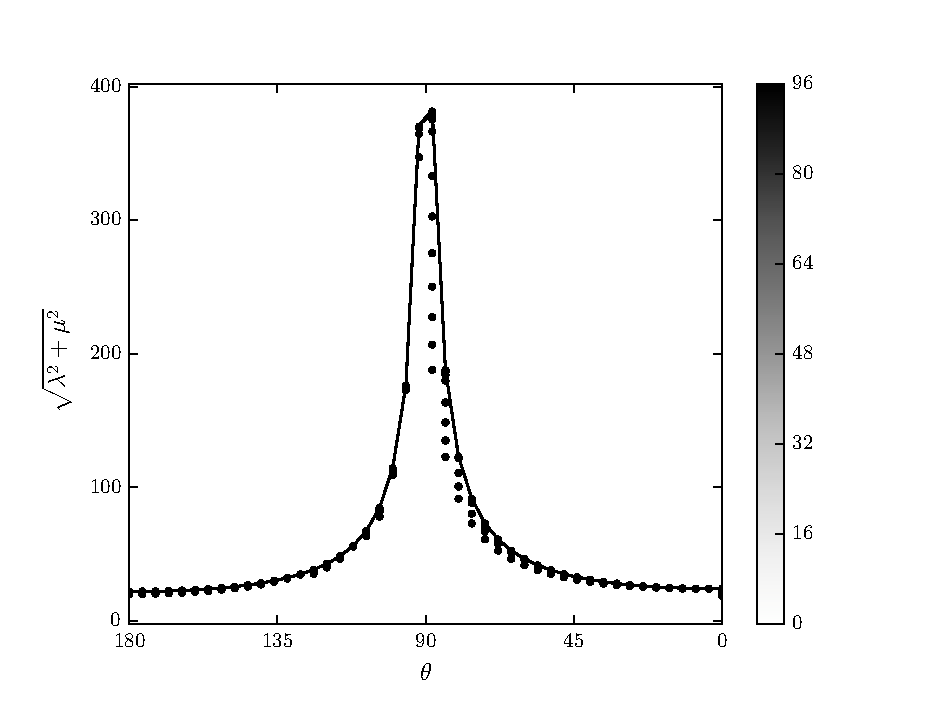
\includegraphics{./fig/ch3/pull/p1/grid.eps}
		\end{center}		
		\caption{Plot of the minimum critical magnitude for detachment as in Figure~\ref{fig:pull:ref}. The bottom substrate is replaced with a continuum of particles, that is the vdW interaction is integrated over the entire real line. The strength of the continuum vdW interaction is $p=1$.
		\label{fig:pull:p1}}
	\end{figure}
	
	\begin{figure}
		\begin{center}
			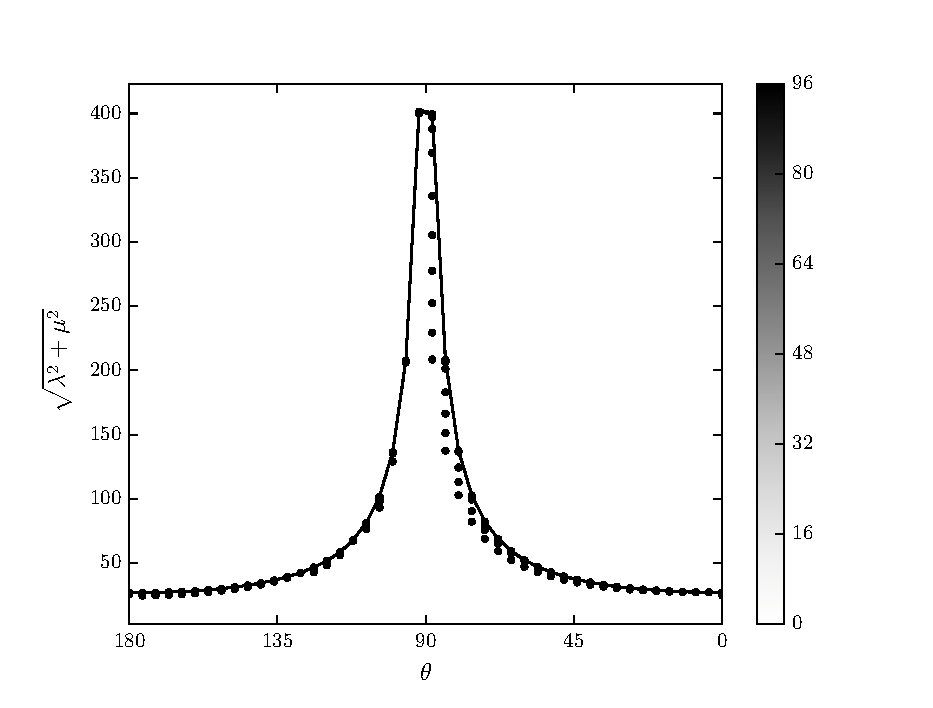
\includegraphics{./fig/ch3/pull/p10/grid.eps}
		\end{center}		
		\caption{Plot of the minimum critical magnitude for detachment as in Figure~\ref{fig:pull:ref}. The bottom substrate is replaced with a continuum of particles. The strength of the continuum vdW interaction is $p=10$.
		\label{fig:pull:p10}}
	\end{figure}

\subsection{Bottom substrate with uniform potential} \label{section:detachment:pressure}

In section~\ref{section:compression:pressure} we replaced the bottom substrate particle-particle potential with a uniform potential. We make the same modification here and briefly discuss the effects on the model under the detachment experiment.

Figure~\ref{fig:pull:p1} and Figure~\ref{fig:pull:p10} show the critical magnitude of the load with the modified bottom substrate potential. The dynamics of the detachment situation are the same as the reference parameters, i.e. that there are two detachment modes: sliding and brute force. There is still a maximum of the critical load near $\theta=90$\textdegree ~and still likely a critical angle were the detachment mode changes. However, the minimums on either side of the plot have changed. An explanation is that there is no resistance for the fiber particles to prevent horizontal displacement because the potential is uniform. Any vertical component of the load does not assist the top substrate in detaching from the fiber which means the minimums on the left and right of the plot should be at $\theta=0$ and $\theta=180$.

	\begin{figure*}
		\centering
		\begin{subfigure}{.5\textwidth}
			\centering
			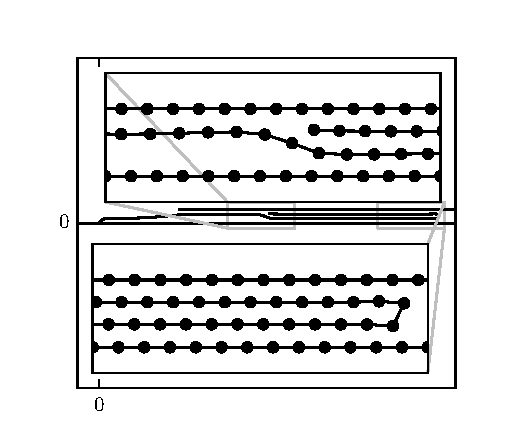
\includegraphics{./fig/ch3/pull/eb0.1/l0_m32.8.eps}
			\caption{$\lambda=0$ and $\mu=32.8$. \label{subfig:folded_over}}
		\end{subfigure}%
		~
		\begin{subfigure}{.5\textwidth}
			\centering
			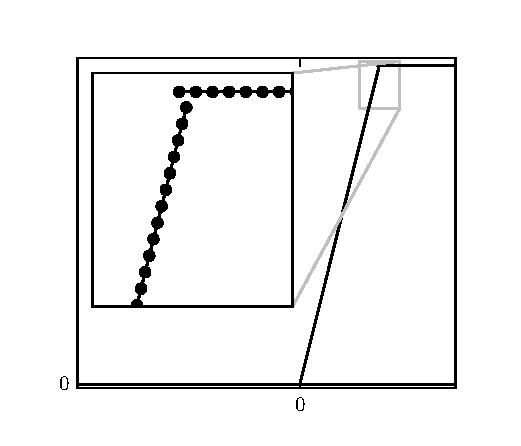
\includegraphics{./fig/ch3/pull/eb0/t76_m4.eps}
			\caption{$\lambda\approx3.88$ and $\mu\approx0.968$\label{subfig:barely_adhered}}
		\end{subfigure}
		\caption{Configuration (a) is an archetypal example of angles of loads on the top substrate that are close to 0. Such loads will often fold ontop of themselves as the top substrate pulls them to the right. Configuration (b) is an archetypal example of the white simulations in the plot for Figure~\ref{fig:pull:eb0}. The reference parameters are modified differently in both examples, for (a) $\eps_-=0.1$ and for (b) $\eps_-=0$.\label{fig:pull_equil}}	
	\end{figure*}

	\begin{figure*}
		\centering
		\begin{subfigure}{.5\textwidth}
			\centering
			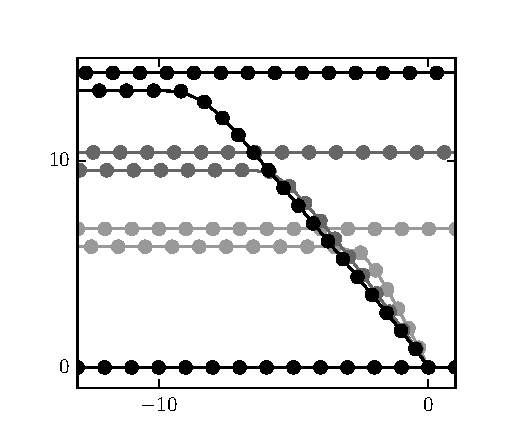
\includegraphics{./fig/ch3/pull/unzip_anim.eps}
			\caption{\label{subfig:unzip}}
		\end{subfigure}%
		~
		\begin{subfigure}{.5\textwidth}
			\centering
			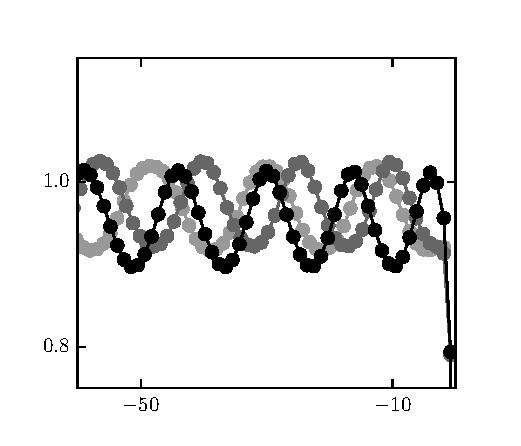
\includegraphics{./fig/ch3/pull/wave_anim.eps}
			\caption{\label{subfig:travel_waves}}
		\end{subfigure}
		\caption{Three time steps of a moving fiber as examples for the kinds of detachemnt modes. Darker fibers are later in the evolution of time. For (a) we see an unzipping mode of detachment were a the top substrate and fiber break the vdW interaction between one particle at a time. For (b) wee see a propogation of waves through a fiber.\label{fig:animation}}	
	\end{figure*}
	